\newpage
\phantomsection
{\bfseries МРНТИ 61.53.91}
\hfill {\bfseries \href{https://doi.org/10.58805/kazutb.v.2.23-409}{https://doi.org/10.58805/kazutb.v.2.23-409}}

\sectionwithauthors{Zh.T. Dauletzhanova, Zh.T.Nurtai}{RESEARCH ON COALS AND ASH RESIDUES FOR THE PRESENCE OF RARE EARTH METALS}

\begin{center}
{\bfseries Zh.T. Dauletzhanova\envelope, Zh.T.Nurtai}

Kazakh University of Technology and Business named after K. Kulazhanov,
Astana, Kazakhstan,

e-mail:Kaliyeva\_zhanna @mail.ru

\envelope Corresponding author: Kaliyeva\_zhanna @mail.ru
\end{center}

This article explores the significance of coal mining and processing
within the framework of the development strategy of the fuel and energy
industry and the transition to a "Green Economy" in the Republic of
Kazakhstan. It emphasizes the underutilized potential of rare metals
present in coal and its by-products and discusses the importance of
developing environmentally friendly technologies for their extraction.
The article highlights the issue of ash slag waste from local thermal
power plants and proposes ways for its rational utilization, including
the extraction of rare metals. The Shubarkol coal deposit in Central
Kazakhstan is considered a significant source of rare metals available
for extraction during coal combustion. The article also underscores the
need for further research and development in this area to maximize the
environmental and economic benefits of using coal resources.

{\bfseries Keywords:} rare metals, coal deposits, ash residues, element
extraction, extraction of valuable metals.

\begin{center}
{\large\bfseries ИССЛЕДОВАНИЯ УГЛЕЙ И ЗОЛООТХОДОВ НА НАЛИЧИЕ РЕДКОЗЕМЕЛЬНЫХ МЕТАЛЛОВ}

{\bfseries Ж.Т., Даулетжанова\envelope, Ж.Т.Нуртай}

Казахский Университет Технологии и Бизнеса имени К. Кулажанова, Астана,
Казахстан,

e-mail: Kaliyeva\_zhanna @mail.ru
\end{center}

Данная статья рассматривает значимость добычи и переработки угля в
контексте стратегии развития топливно-энергетической отрасли и перехода
к "Зеленой экономике" в Республике Казахстан. Она подчеркивает
неиспользованный потенциал редких металлов, содержащихся в угле и его
отходах, и обсуждает важность разработки экологически чистых технологий
для их извлечения. В статье выделяется проблема золошлаковых отходов от
местных тепловых электростанций и предлагаются пути их рационального
использования, включая извлечение редких металлов. Шубаркольское
угольное месторождение в Центральном Казахстане рассматривается как
значительный источник редких металлов, доступных для извлечения в
процессе сжигания угля. Статья также подчеркивает необходимость
дальнейших исследований и разработок в этой области для максимизации
экологических и экономических выгод от использования угольных ресурсов.

{\bfseries Ключевые слова:} редкие металлы, угольные месторождения,
золоотходы, экстракция элементов, извлечение ценных металлов.

\begin{center}
{\large\bfseries ҚЫЗЫҒУШЫ ҚҰРЫЛТАЙЛАР МЕН ҚЫЗЫҒУШЫ АСТАРҒА АРНАЛҒАН ҚАЗЫНАЛАРДЫҢ
ТАЛДАУЫ ЖӘНЕ ТҰТАСТАРДЫҢ РЕДКІ МЕТАЛДАРЫНЫҢ БАРЛЫҚТЫҚТАРЫН ТЕКСЕРУ}

{\bfseries Ж.Т. Даулетжанова\envelope, Ж.Т.Нұртай}

К. Құлажанов атындағы Қазақ Технология және Бизнес Университеті, Астана,
Қазақстан,

e-mail:Kaliyeva\_zhanna @mail.ru
\end{center}

Бұл мақалада Қазақстан Республикасының топтық-энергиялық саладағы даму
стратегиясы және "Жасыл экономика"ға көшу концепциясы контекстінде көмір
екімі мен өңдеу маңыздылығы тексеріледі. Бұл мақала көмір мен оның жалға
материалдарындағы талаптары қолданылмаған қызметті мөлшерлердің бойынша
көмір мен оның толқындарындағы күндізгі металлдардың көрсеткіштілігін
негіздеуге қарсы ерекше технологияларды дамыту маңыздылығын айқындайды.
Мақала орта маңызды термалды энергиялық станциялардың местік қызметінен
шығатын мал бұзылу мүлдеміні талқау және бұның рақсетті пайдалануларын
көру үрдісіне ықпал етеді, оның ішінде редкі металдарды шығаруларын
қоспаған. Ортағасы Қазақстандағы Шубарқол көмір местінен мәні шамамен
көмірдің жауқындысы кезінде шығаруға болатын қызметті металлдардың
маңызды құрылымы ретінде сипатталады. Мақала көмір ресурстарын
қолдануның экологиялық және экономикалық маңыздылығын көмек көрсету үшін
осы жағдайда кейбір басқармаларда үздіктіктер мен зерттеулерді өткізу
керектігін түсіндіреді.

{\bfseries Tүйін сөздер:} сирек металдар, көмір кен орындары, күл
қалдықтары, элементтерді шығару, бағалы металдарды алу.

\begin{multicols}{2}
{\bfseries Introduction.} In accordance with the Development Concept of the
Fuel and Energy Industry of the Republic of Kazakhstan for the period up
to 2030 and the implementation of the Concept for Transition to a "Green
Economy," the expansion of coal usage should serve as an incentive for
conducting research and development of new, environmentally friendly
technologies for its extraction, combustion, and processing {[}1{]}.

Currently, coal mining and comprehensive processing are gaining
increasing importance due to the potential utilization of previously
non-commercial deposits. The search and development of rare earth
metals, as well as the utilization of waste from black and non-ferrous
metallurgy production, play a significant role in the rational use of
natural resources. One of the goals of this study is to address this
issue. One possible approach to its solution is the utilization of waste
as a source of rare earth metals {[}2,3{]}.

Currently, the rare-metal potential of coals is practically untapped.
From coals and their wastes on an industrial scale, only germanium (Ge)
and gold (Au) are extracted. Technologies for extracting gallium (Ga),
scandium (Sc), rare earth metals, and some other metals have also been
developed.

From the perspective of rational land use, coals and their combustion
products represent raw materials extracted from the
earth\textquotesingle s depths, which are transported to other
territories and inadequately utilized to satisfy many industrial needs
{[}4{]}.

Ash dumps formed at local thermal power plants pose a serious
environmental threat to the region and can have a negative impact on the
environment and human health. Due to wind erosion, ash particles can
enter the atmosphere and spread over long distances, leading to air
pollution. Settled dust, accompanied by chemically active toxic
substances, can contaminate soil. Moreover, under the influence of acid
rain, toxic substances from ash dumps are mobilized, which can lead to
soil, groundwater, and surface water pollution.

In light of the above, it becomes evident that ash dumps cause
significant environmental, economic, and social damage to the region.
The problem of ash slag material utilization requires immediate solution
{[}5{]}.

Currently, in global practice, coal deposits are increasingly being
considered not only as a source of fuel and energy raw materials but
also as a potential source of a range of rare elements and noble metals
(including the USA, China, Russia, and other countries). Partial studies
of the composition of rare metals in coal organic materials have been
conducted in developed economies (USA, Europe, Australia, China),
reflected in numerous scientific publications. These studies indicate
that coal industry wastes may contain high concentrations of rare
elements, which in some cases may be industrially significant.

However, existing methods for extracting rare metals currently have low
efficiency, not exceeding 30\%. This limits the attractiveness of
investments in the development of domestic processing industries
{[}6{]}.

The current global annual volume of gold slag waste (GSW) extraction is
approximately 750 million tons, and an increase in this volume is
expected in the near future.

{\bfseries Materials and methods.} Methods of detecting rare earth metals:
Mass spectrometry (MS); atomic emission spectrometry (AES); X-ray
fluorescence analysis (XRF); laser diffraction method.

Mass spectrometry (MS) is based on the ionization of the sample
substance in a magnetic field. The ions are subjected to the Lorentz
force, the magnitude of which depends on the mass and charge of the ion.
The difference in the trajectories of different ions allows for the
determination of the atomic content of substances in the sample. To
perform measurements, the sample of the investigated solid substance
needs to be decomposed to eliminate factors that distort the analysis
data and converted into a solution, which is labor-intensive and
time-consuming {[}7{]}.

The sensitivity of this method significantly depends on the ionization
method and the detectors used. According to {[}8,9{]}, when using an
inductively coupled plasma mass spectrometer (ICP-MS) to determine the
concentration of rare earth elements (REEs) in solution, the sensitivity
is about 10-12 mg/L. The accuracy of the method depends on the
concentration of the determined element (C) in the sample; polyatomic
interferences and matrix effects also introduce errors {[}10{]}.
Interfering impurities include ions with the same mass-to-charge ratio
as the determined atom, as well as certain isotopes; for example, for
La, these are LaO+, LaOH+, and 155Gd+ {[}7{]}. According to
Panteeva\textquotesingle s data {[}11{]}, as the value of C decreases
from 1000 g/t to 0.01 g/t, the measurement error increases from 8\% to
32\%. The reproducibility of the method is considered good {[}7{]}, but
it may also decrease as the value of C decreases. Therefore, the
considered method is expedient to use for determining relatively high
(tens and hundreds of g/t) concentrations of elements in ash and with
relatively small fluctuations over time in the elemental composition of
the analyzed ash.
\end{multicols}

\begin{figure}[H]
	\centering
	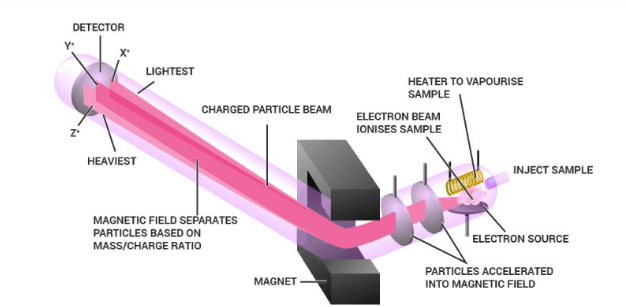
\includegraphics[width=0.8\textwidth]{assets/1049}
	\caption*{Figure 1 - Operation of Mass Spectrometer: Principle and Schematic Diagram of the Spectrometer}
\end{figure}

\begin{multicols}{2}
Atomic emission spectrometry (AES) is a method based on the emission of
electromagnetic radiation by excited atoms or ions. To achieve this, the
sample substance is subjected to high temperatures, resulting in the
dissociation of compounds into atoms and an increase in the number of
collisions leading to the ionization of atoms. Atoms and ions, being in
an excited state, are capable of returning to their ground energy state
by transferring thermal or radiative energy and emitting electromagnetic
radiation. This allows for the determination of the quantity of atoms,
and consequently, the concentrations of elements. The emission spectrum
of an element contains more lines than its corresponding absorption
spectrum.

For measurements, similar to the MS method, the sample of the solid
substance is converted into a solution and heated to evaporate the
solvent and excite the atoms of the investigated substance {[}12{]}. The
emitted radiation from the atoms is decomposed into a spectrum and
recorded. For qualitative analysis, spectral lines are identified, and
for quantitative analysis of elements, the intensity of the lines is
measured. The concentration of elements is determined using
pre-established calibration graphs. The error is caused by the overlap
of spectral lines of different elements, as well as the matrix effect.
According to data, the relative standard deviation (RSD) during the
analysis of geological materials ranges from 5\% (Y, Eu) to 10\% (Pr).
Interfering elements include: Na, K, Ca, Fe. It is also noted that light
REEs, such as La, Nd, Ce, Pr, Sm, interfere with the determination of
heavy REEs, such as Ho, Er, Tm, Yb, Lu, so separate determination of
these groups of REEs is recommended. Zybinski et al. showed that for La,
Ce, Eu, Y, Gd, the systematic error of determination does not exceed
5\%; for Lu, Yb, Ho, Sc - no more than 15\%; for Dy, Er, Tm, Nd - no
more than 25\%; for Pr, Sm, Tb - tens and hundreds of percent. The
reproducibility and repeatability of AES with an element content above
100 g/t is no more than 5\%, less than 100 g/t - no more than 10\%
{[}13{]}. The detection limits of some REEs, in g/t: Y - 2; Zr - 4; La -
2000; Ce - 4000; Pr - 30; Nd - 20; Eu - 1; Dy - 5; Er - 8. From the
presented data, it can be seen that the accuracy and sensitivity of this
method for different REEs vary significantly. Therefore, the application
of AES is advisable for the determination of elements in ash such as Y,
Zr, Dy, Er. At the same time, for a complete analysis of REE content, it
is preferable to combine MS and AES methods.
\end{multicols}

\begin{figure}[H]
	\centering
	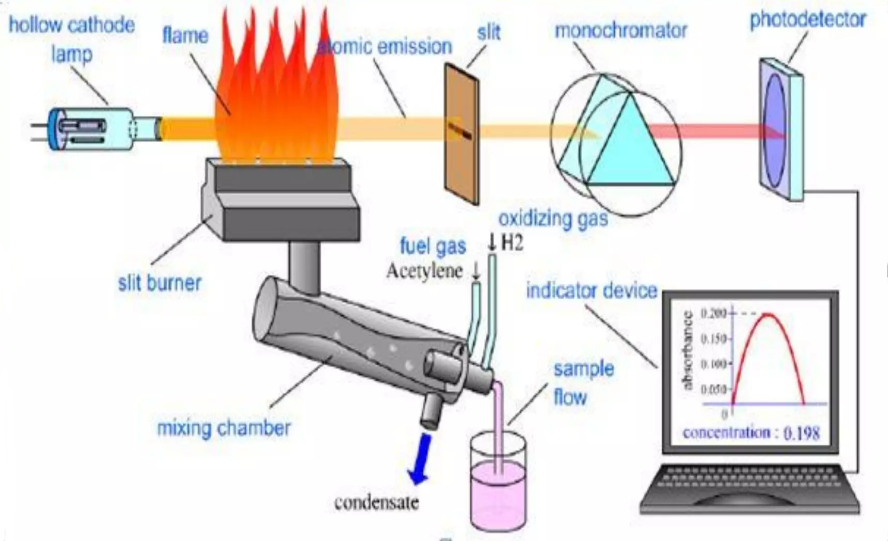
\includegraphics[width=0.8\textwidth]{assets/1050}
	\caption*{Figure 2 - X-ray Fluorescence Analysis (XRF)}
\end{figure}

\begin{multicols}{2}
X-ray Fluorescence Analysis (XRF) is based on the analysis of the
spectrum generated by using X-ray radiation {[}7{]}.

When interacting with high-energy photons, atoms of the substance
transition to an excited state, resulting in electron transitions from
lower orbitals to higher energy levels up to ionization of the atom. In
the excited state, the atom remains for a very short time, about one
microsecond, after which it returns to its ground state. During this
process, electrons from outer shells fill the vacant positions, and the
excess energy is either emitted as a photon or transferred to another
electron from the outer shells. Each atom emits a quantum with energy of
a strictly defined value. The substance structure is judged by the
energy and quantity of quanta emitted.

There are several variations of this method:

Wavelength dispersion is used to determine the concentrations of
impurity elements; characterized by relatively high sensitivity;

Energy-dispersive method is less sensitive but more suitable for express
analysis {[}10{]}.

The sensitivity of the method in determining the concentration of REEs
in solid materials is at the level of the Clarke content of the element.
The method error depends on the nature of the element and its
concentration. Thus, according to {[}14{]}, when determining Y, La, Ce,
Pr, and Nd, it ranged from 18 to 28\%. Reproducibility is about a few
percent. According to {[}7{]}, the accuracy and reproducibility of the
results increase due to pressing the investigated powder material and
melting with lithium tetraborate.

Compared to the methods described above, XRF is characterized by less
complexity because the material does not need to be decomposed and
converted into a solution. The time required for the analysis is
relatively short, amounting to several minutes. Disadvantages include
relatively low accuracy and the inability to determine the concentration
of elements with an atomic mass of less than 40 a.m.u. This method is
acceptable for the express assessment of REE content in ash. Other
methods of determining the REE content are also mentioned in the
literature. In particular, neutron activation analysis, which, according
to {[}7{]}, was effective for determining La, Ce, Nd, Sm, Eu, Tb, Yb, Lu
in the 1960s - 1980s but was then replaced by the more accurate and
versatile MS method. The radiometric method, due to its low complexity
and speed, has found wide application for the analysis of the elemental
composition of ores, but the low sensitivity (about several hundred g/t)
makes it impossible to apply this method for most REEs.
\end{multicols}

\begin{figure}[H]
	\centering
	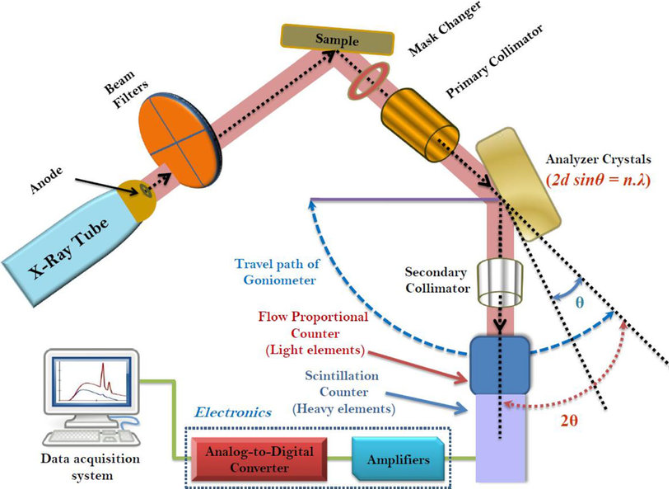
\includegraphics[width=0.6\textwidth]{assets/1051}
	\caption*{Figure 3 - X-ray Fluorescence Spectrometer}
\end{figure}

\begin{multicols}{2}
Laser Diffraction Method. Unlike the previous method, it involves the
use of laser instead of visible light {[}12{]}. This allows measurements
of particle diameters in the range from 10 nm to 3500 μm, corresponding
to the particle size of ash. The accuracy of the method, according to
{[}15{]}, ranges from 1 to 4\%. Advantages include a wide range of
measurements, high measurement accuracy, speed, simplicity, the
possibility of measurements in a flow-through mode, and good
reproducibility. Disadvantages include difficulty in detecting particles
at low concentrations and the need to disperse particles in a liquid
{[}7{]}.

{\bfseries Results and discussion}. The Shubarkol deposit in Central
Kazakhstan has reserves of more than 1 billion tons. These are
significant sources of rare earths that can be extracted during coal
combustion at thermal power plants (TPPs). Coal deposits contain 64 g/t
of scandium, 384 g/t of dysprosium, and 335 g/t of gadolinium (see
Figure 4). Thus, these are large reserves of rare earths available for
extraction during the coal combustion process at TPPs.
\end{multicols}

\begin{figure}[H]
	\centering
	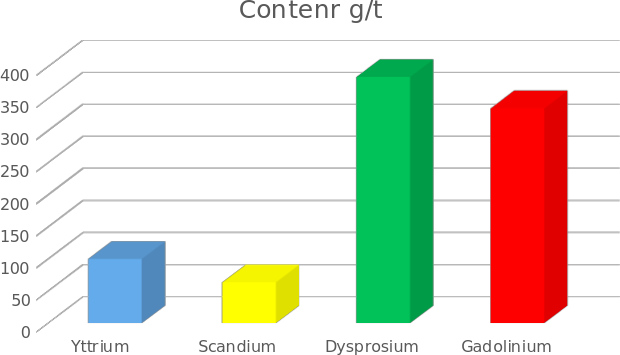
\includegraphics[width=0.6\textwidth]{assets/1083}
	\caption*{Figure 4 - Rare Earth Element Content in Shubarkol Coal Deposit}
\end{figure}

\begin{multicols}{2}
The advantages of using waste as resources have both environmental and
economic aspects:

It is one of the most rational ways to address environmental issues as
it helps reduce anthropogenic pressure on the natural environment.

Waste processing contributes to increasing the economic efficiency of
thermal power plants.

As a result of secondary waste processing, companies can reduce expenses
on slag and ash storage, and also utilize them as a source of rare and
rare earth metals, leading to additional economic benefits.

Surface waste does not require additional extraction expenses, which is
a positive factor for geological enterprises. This also contributes to
increasing extraction volumes with maximum useful component extraction
and reducing the areas alienated for deposit development. In this
context, coal ash generated during combustion can be considered as
potential ore from which rare earth metals can be extracted in the
future. The concentration of these metals in ash can serve as an
important indicator for industrial deposit assessment {[}16{]}.
\end{multicols}

\begin{table}[H]
\caption*{Table 1 - Rare Earth Content in Coals from Various Geological and Industrial Districts of the Kuzbass Region}
\centering
\begin{tabular}{|l|lllllllll|}
\hline
\multirow{2}{*}{Geological-industrial area} & \multicolumn{9}{l|}{Element} \\ \cline{2-10}
 & \multicolumn{1}{l|}{N} & \multicolumn{1}{l|}{La} & \multicolumn{1}{l|}{Ce} & \multicolumn{1}{l|}{Sm} & \multicolumn{1}{l|}{Eu} & \multicolumn{1}{l|}{Tb} & \multicolumn{1}{l|}{Yb} & \multicolumn{1}{l|}{Lu} & Yb \\ \hline
Angers & \multicolumn{1}{l|}{2} & \multicolumn{1}{l|}{1,8} & \multicolumn{1}{l|}{3,9} & \multicolumn{1}{l|}{0,7} & \multicolumn{1}{l|}{0,1} & \multicolumn{1}{l|}{0,2} & \multicolumn{1}{l|}{0,35} & \multicolumn{1}{l|}{0,15} & 5,1 \\ \hline
Aralichevsky & \multicolumn{1}{l|}{122} & \multicolumn{1}{l|}{17,6} & \multicolumn{1}{l|}{29,8} & \multicolumn{1}{l|}{3,05} & \multicolumn{1}{l|}{1,31} & \multicolumn{1}{l|}{0,58} & \multicolumn{1}{l|}{1,78} & \multicolumn{1}{l|}{0,38} & 9,9 \\ \hline
Baydaevsky & \multicolumn{1}{l|}{10} & \multicolumn{1}{l|}{18,3} & \multicolumn{1}{l|}{28,2} & \multicolumn{1}{l|}{2,9} & \multicolumn{1}{l|}{1,03} & \multicolumn{1}{l|}{0,53} & \multicolumn{1}{l|}{2,1} & \multicolumn{1}{l|}{0,41} & 8,7 \\ \hline
Bachatsky & \multicolumn{1}{l|}{5} & \multicolumn{1}{l|}{24,5} & \multicolumn{1}{l|}{12,7} & \multicolumn{1}{l|}{3,42} & \multicolumn{1}{l|}{1,18} & \multicolumn{1}{l|}{0,15} & \multicolumn{1}{l|}{1,68} & \multicolumn{1}{l|}{0,25} & 14,6 \\ \hline
Bunguro-Chumyshsky & \multicolumn{1}{l|}{9} & \multicolumn{1}{l|}{13,9} & \multicolumn{1}{l|}{25,6} & \multicolumn{1}{l|}{2,37} & \multicolumn{1}{l|}{0,65} & \multicolumn{1}{l|}{0,37} & \multicolumn{1}{l|}{0,89} & \multicolumn{1}{l|}{0,39} & 15,6 \\ \hline
Kemerovo & \multicolumn{1}{l|}{116} & \multicolumn{1}{l|}{9,9} & \multicolumn{1}{l|}{23,9} & \multicolumn{1}{l|}{2,33} & \multicolumn{1}{l|}{0,6} & \multicolumn{1}{l|}{0,56} & \multicolumn{1}{l|}{1,06} & \multicolumn{1}{l|}{0,27} & 9,3 \\ \hline
Kondomsky & \multicolumn{1}{l|}{9} & \multicolumn{1}{l|}{16,8} & \multicolumn{1}{l|}{26,2} & \multicolumn{1}{l|}{3,23} & \multicolumn{1}{l|}{0,93} & \multicolumn{1}{l|}{0,99} & \multicolumn{1}{l|}{2,19} & \multicolumn{1}{l|}{0,63} & 7,7 \\ \hline
Leninist & \multicolumn{1}{l|}{18} & \multicolumn{1}{l|}{7,9} & \multicolumn{1}{l|}{17,7} & \multicolumn{1}{l|}{1,33} & \multicolumn{1}{l|}{0,33} & \multicolumn{1}{l|}{0,2} & \multicolumn{1}{l|}{1,13} & \multicolumn{1}{l|}{0,33} & 7 \\ \hline
Mrassky & \multicolumn{1}{l|}{73} & \multicolumn{1}{l|}{24,7} & \multicolumn{1}{l|}{37,9} & \multicolumn{1}{l|}{2,94} & \multicolumn{1}{l|}{0,78} & \multicolumn{1}{l|}{0,58} & \multicolumn{1}{l|}{3,02} & \multicolumn{1}{l|}{2,09} & 8,2 \\ \hline
Osinnikovsky & \multicolumn{1}{l|}{56} & \multicolumn{1}{l|}{8} & \multicolumn{1}{l|}{15,8} & \multicolumn{1}{l|}{2,05} & \multicolumn{1}{l|}{0,42} & \multicolumn{1}{l|}{1,02} & \multicolumn{1}{l|}{0,8} & \multicolumn{1}{l|}{0,33} & 10 \\ \hline
Prokopyevsky & \multicolumn{1}{l|}{140} & \multicolumn{1}{l|}{8,4} & \multicolumn{1}{l|}{14,3} & \multicolumn{1}{l|}{1,41} & \multicolumn{1}{l|}{0,31} & \multicolumn{1}{l|}{0,19} & \multicolumn{1}{l|}{1,57} & \multicolumn{1}{l|}{0,26} & 5,3 \\ \hline
Tom-Usinsky & \multicolumn{1}{l|}{169} & \multicolumn{1}{l|}{12,2} & \multicolumn{1}{l|}{22,6} & \multicolumn{1}{l|}{2,5} & \multicolumn{1}{l|}{0,41} & \multicolumn{1}{l|}{0,75} & \multicolumn{1}{l|}{1,37} & \multicolumn{1}{l|}{0,28} & 8,9 \\ \hline
Uskatsky & \multicolumn{1}{l|}{15} & \multicolumn{1}{l|}{12,6} & \multicolumn{1}{l|}{38,8} & \multicolumn{1}{l|}{5,1} & \multicolumn{1}{l|}{0,87} & \multicolumn{1}{l|}{-} & \multicolumn{1}{l|}{1,1} & \multicolumn{1}{l|}{-} & 11,5 \\ \hline
\end{tabular}
\end{table}

\begin{figure}[H]
	\centering
	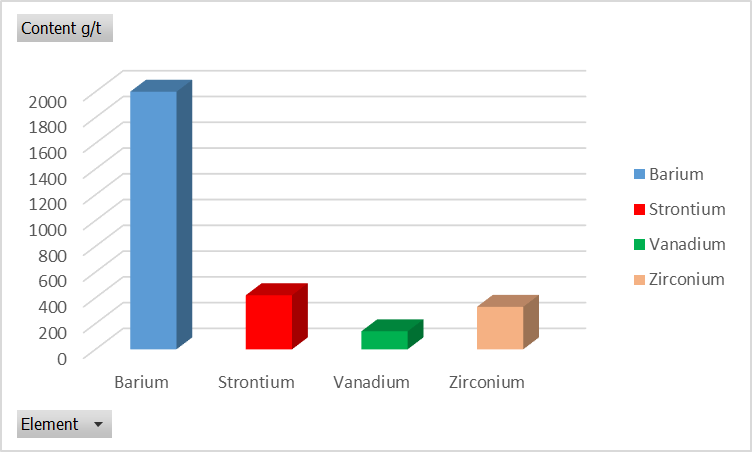
\includegraphics[width=0.7\textwidth]{assets/1052}
	\caption*{Figure 5 - Results of neutron activation analysis of fly ash}
\end{figure}

\begin{multicols}{2}
Characterization of Fly Ash from Ekibastuz Coal as Raw Material for Deep
Processing includes an analysis of the composition obtained from the
electrostatic precipitators of Omsk TPP-4. The main components comprise
silicon, aluminum, and iron oxides, reaching up to 95\%. Additionally,
the fly ash contains oxides of alkali and alkaline-earth metals, with a
total content of 2.3\%. Moreover, the presence of 15 trace elements,
each exceeding 10-4\%, has been identified.
\end{multicols}

\begin{table}[H]
\caption*{Table 2 - Chemical Composition of Fly Ash from the Ekibastuz Coal Basin}
\centering
\begin{tabular}{|l|l|l|l|l|l|l|l|l|l|l|}
\hline
SiO\tsb{2} & AI\tsb{2}O\tsb{3} & Fe\tsb{2}O\tsb{3} & CaO & MgO & TiO\tsb{2} & K2O & Na\tsb{2}O & P2O\tsb{5} & MnO\tsb{2} & SO\tsb{3} \\ \hline
61,5 & 27,4 & 5,65 & 1,17 & 0,49 & 1,49 & 0,42 & 0,32 & 0,52 & 0,17 & 0,57 \\ \hline
\end{tabular}
\end{table}

\begin{table}[H]
\caption*{Table 3 - Elements of ash slag waste from the Shubarkol coal deposit classified as rare are debated}
\centering
\resizebox{\textwidth}{!}{%
\begin{tabular}{|lll|llllllll|p{0.13\textwidth}|}
\hline
\multicolumn{3}{|l|}{\textbf{Sample №}} & \multicolumn{1}{l|}{№1} & \multicolumn{1}{l|}{№2} & \multicolumn{1}{l|}{№3} & \multicolumn{1}{l|}{№4} & \multicolumn{1}{l|}{№5} & \multicolumn{1}{l|}{\textbf{Ср}} & \multicolumn{1}{l|}{\textbf{Min}} & \textbf{Max} & \multirow{2}{=}{\textbf{Price million tenge/gram}} \\ \cline{1-11}
\multicolumn{3}{|l|}{\textbf{Element}} & \multicolumn{8}{l|}{\textbf{Content, g/ton}} &  \\ \hline
\multicolumn{1}{|l|}{1} & \multicolumn{1}{l|}{Boron} & B & \multicolumn{1}{l|}{100} & \multicolumn{1}{l|}{200} & \multicolumn{1}{l|}{160} & \multicolumn{1}{l|}{140} & \multicolumn{1}{l|}{100} & \multicolumn{1}{l|}{140} & \multicolumn{1}{l|}{100} & 200 & 315 \\ \hline
\multicolumn{1}{|l|}{2} & \multicolumn{1}{l|}{Strontium} & Sr & \multicolumn{1}{l|}{400} & \multicolumn{1}{l|}{280} & \multicolumn{1}{l|}{220} & \multicolumn{1}{l|}{172} & \multicolumn{1}{l|}{490} & \multicolumn{1}{l|}{312,4} & \multicolumn{1}{l|}{172} & 490 & 7,92 \\ \hline
\multicolumn{1}{|l|}{3} & \multicolumn{1}{l|}{Selenium} & Se & \multicolumn{1}{l|}{0,6} & \multicolumn{1}{l|}{0,6} & \multicolumn{1}{l|}{0,6} & \multicolumn{1}{l|}{0,6} & \multicolumn{1}{l|}{0,6} & \multicolumn{1}{l|}{0,6} & \multicolumn{1}{l|}{0,6} & 0,6 & 6,44 \\ \hline
\multicolumn{1}{|l|}{4} & \multicolumn{1}{l|}{Tellurium} & Te & \multicolumn{1}{l|}{0,06} & \multicolumn{1}{l|}{0,06} & \multicolumn{1}{l|}{0,06} & \multicolumn{1}{l|}{0,06} & \multicolumn{1}{l|}{0,06} & \multicolumn{1}{l|}{0,06} & \multicolumn{1}{l|}{0,06} & 0,06 & 3,47 \\ \hline
\multicolumn{1}{|l|}{5} & \multicolumn{1}{l|}{Bismuth} & Bi & \multicolumn{1}{l|}{60} & \multicolumn{1}{l|}{60} & \multicolumn{1}{l|}{60} & \multicolumn{1}{l|}{60} & \multicolumn{1}{l|}{60} & \multicolumn{1}{l|}{60} & \multicolumn{1}{l|}{60} & 60 & 2,25 \\ \hline
\multicolumn{1}{|l|}{6} & \multicolumn{1}{l|}{Cadmium} & Cd & \multicolumn{1}{l|}{18800} & \multicolumn{1}{l|}{19200} & \multicolumn{1}{l|}{9900} & \multicolumn{1}{l|}{20600} & \multicolumn{1}{l|}{10000} & \multicolumn{1}{l|}{15700} & \multicolumn{1}{l|}{9900} & 20600 & 1,39 \\ \hline
\end{tabular}
}
\end{table}

\begin{table}[H]
\caption*{Table 4 - Rare Earth Elements Present in the Shubarkol Coal Deposit}
\centering
\resizebox{\textwidth}{!}{%
\begin{tabular}{|lll|llllllll|p{0.13\textwidth}|}
\hline
\multicolumn{3}{|l|}{\textbf{Sample №}} & \multicolumn{1}{l|}{№1} & \multicolumn{1}{l|}{№2} & \multicolumn{1}{l|}{№3} & \multicolumn{1}{l|}{№4} & \multicolumn{1}{l|}{№5} & \multicolumn{1}{l|}{\textbf{Average}} & \multicolumn{1}{l|}{\textbf{Min}} & \textbf{Max} & \multirow{2}{=}{\textbf{Price million tenge/gram}} \\ \cline{1-11}
\multicolumn{3}{|l|}{\textbf{Element}} & \multicolumn{8}{l|}{\textbf{Content, g/ton}} &  \\ \hline
\multicolumn{1}{|l|}{1} & \multicolumn{1}{l|}{Scandium} & Sc & \multicolumn{1}{l|}{20} & \multicolumn{1}{l|}{20} & \multicolumn{1}{l|}{20} & \multicolumn{1}{l|}{20} & \multicolumn{1}{l|}{20} & \multicolumn{1}{l|}{20} & \multicolumn{1}{l|}{20} & 20 & 292,5 \\ \hline
\multicolumn{1}{|l|}{2} & \multicolumn{1}{l|}{Yttrium} & Y & \multicolumn{1}{l|}{6} & \multicolumn{1}{l|}{13} & \multicolumn{1}{l|}{7} & \multicolumn{1}{l|}{33} & \multicolumn{1}{l|}{11} & \multicolumn{1}{l|}{14} & \multicolumn{1}{l|}{6} & 33 & 198 \\ \hline
\multicolumn{1}{|l|}{3} & \multicolumn{1}{l|}{Germanium} & Ge & \multicolumn{1}{l|}{7} & \multicolumn{1}{l|}{7} & \multicolumn{1}{l|}{7} & \multicolumn{1}{l|}{7} & \multicolumn{1}{l|}{7} & \multicolumn{1}{l|}{7} & \multicolumn{1}{l|}{7} & 7 & 134,55 \\ \hline
\multicolumn{1}{|l|}{4} & \multicolumn{1}{l|}{Lanthanum} & La & \multicolumn{1}{l|}{34} & \multicolumn{1}{l|}{93} & \multicolumn{1}{l|}{52} & \multicolumn{1}{l|}{140} & \multicolumn{1}{l|}{48} & \multicolumn{1}{l|}{73,4} & \multicolumn{1}{l|}{34} & 140 & 99 \\ \hline
\multicolumn{1}{|l|}{5} & \multicolumn{1}{l|}{Beryllium} & Be & \multicolumn{1}{l|}{4} & \multicolumn{1}{l|}{4} & \multicolumn{1}{l|}{7} & \multicolumn{1}{l|}{17} & \multicolumn{1}{l|}{10} & \multicolumn{1}{l|}{8,4} & \multicolumn{1}{l|}{4} & 17 & 46,58 \\ \hline
\multicolumn{1}{|l|}{6} & \multicolumn{1}{l|}{Niobium} & Nb & \multicolumn{1}{l|}{10} & \multicolumn{1}{l|}{10} & \multicolumn{1}{l|}{10} & \multicolumn{1}{l|}{10} & \multicolumn{1}{l|}{10} & \multicolumn{1}{l|}{10} & \multicolumn{1}{l|}{10} & 10 & 35,69 \\ \hline
\multicolumn{1}{|l|}{7} & \multicolumn{1}{l|}{Vanadium} & V & \multicolumn{1}{l|}{57} & \multicolumn{1}{l|}{79} & \multicolumn{1}{l|}{110} & \multicolumn{1}{l|}{270} & \multicolumn{1}{l|}{88} & \multicolumn{1}{l|}{120,8} & \multicolumn{1}{l|}{57} & 270 & 34,65 \\ \hline
\multicolumn{1}{|l|}{8} & \multicolumn{1}{l|}{Indium} & In & \multicolumn{1}{l|}{0,09} & \multicolumn{1}{l|}{0,09} & \multicolumn{1}{l|}{0,09} & \multicolumn{1}{l|}{0,09} & \multicolumn{1}{l|}{0,09} & \multicolumn{1}{l|}{0,09} & \multicolumn{1}{l|}{0,09} & 0,09 & 18,09 \\ \hline
\multicolumn{1}{|l|}{9} & \multicolumn{1}{l|}{Zirconium} & Zr & \multicolumn{1}{l|}{30} & \multicolumn{1}{l|}{50} & \multicolumn{1}{l|}{30} & \multicolumn{1}{l|}{70} & \multicolumn{1}{l|}{30} & \multicolumn{1}{l|}{42} & \multicolumn{1}{l|}{30} & 70 & 10,89 \\ \hline
\multicolumn{1}{|l|}{10} & \multicolumn{1}{l|}{Lithium} & Li & \multicolumn{1}{l|}{45} & \multicolumn{1}{l|}{45} & \multicolumn{1}{l|}{45} & \multicolumn{1}{l|}{45} & \multicolumn{1}{l|}{45} & \multicolumn{1}{l|}{45} & \multicolumn{1}{l|}{45} & 45 & 9,9 \\ \hline
\multicolumn{1}{|l|}{11} & \multicolumn{1}{l|}{Molybdenum} & Mo & \multicolumn{1}{l|}{3} & \multicolumn{1}{l|}{4} & \multicolumn{1}{l|}{4} & \multicolumn{1}{l|}{11} & \multicolumn{1}{l|}{3} & \multicolumn{1}{l|}{5} & \multicolumn{1}{l|}{3} & 11 & 7,92 \\ \hline
\multicolumn{1}{|l|}{12} & \multicolumn{1}{l|}{Titanium} & Ti & \multicolumn{1}{l|}{1200} & \multicolumn{1}{l|}{3300} & \multicolumn{1}{l|}{2100} & \multicolumn{1}{l|}{780} & \multicolumn{1}{l|}{2700} & \multicolumn{1}{l|}{2016} & \multicolumn{1}{l|}{780} & 3300 & 7,57 \\ \hline
\multicolumn{1}{|l|}{13} & \multicolumn{1}{l|}{Thallium} & Tl & \multicolumn{1}{l|}{0,2} & \multicolumn{1}{l|}{0,3} & \multicolumn{1}{l|}{0,1} & \multicolumn{1}{l|}{0,3} & \multicolumn{1}{l|}{0,1} & \multicolumn{1}{l|}{0,2} & \multicolumn{1}{l|}{0,1} & 0,3 & 7,43 \\ \hline
\multicolumn{1}{|l|}{14} & \multicolumn{1}{l|}{Tellurium} & Te & \multicolumn{1}{l|}{0,06} & \multicolumn{1}{l|}{0,06} & \multicolumn{1}{l|}{0,06} & \multicolumn{1}{l|}{0,06} & \multicolumn{1}{l|}{0,06} & \multicolumn{1}{l|}{0,06} & \multicolumn{1}{l|}{0,06} & 0,06 & 3,47 \\ \hline
\multicolumn{1}{|l|}{15} & \multicolumn{1}{l|}{Tungsten} & W & \multicolumn{1}{l|}{5} & \multicolumn{1}{l|}{5} & \multicolumn{1}{l|}{6} & \multicolumn{1}{l|}{5} & \multicolumn{1}{l|}{5} & \multicolumn{1}{l|}{5,2} & \multicolumn{1}{l|}{5} & 6 & 3,47 \\ \hline
\end{tabular}%
}
\end{table}

\begin{multicols}{2}
Rare metals present the greatest potential as they do not form their own
deposits. Among the rare metals contained in this fly ash, the following
groups are distinguished: dispersed - Ga; refractory - Ti, Zr, V; rare
earth - Y, Yb, Tb, La, Ce, Dy, Sm; radioactive - U, Th.

The phase composition of the ash also plays an important role in the
efficiency of element extraction. X-ray phase analysis, conducted on the
Drone-3 setup using the Kα line and p-filter, revealed the presence of
an amorphous phase in the ash, as well as alpha-quartz and
aluminosilicates of the sillimanite type
Al\textsubscript{2}O\textsubscript{3}xSiO\textsubscript{2} or mullite
3Al\textsubscript{2}O\textsubscript{3}x2SiO\textsubscript{2}. The
fundamental principles of silicon and aluminum extraction during
hydroprocessing were studied, allowing for the complete separation of
the amorphous phase {[}17-18{]}.

During the oxidation of coal seams and coal combustion, a significant
portion of rare earth metals transitions into the composition of
combustion gas products or settles in the gas cleaning system. At the
same time, the concentration of these metals in ash slag waste exceeds
their content in the original coal materials. For example, the gold
content in ash slag waste after coal combustion may exceed the gold
content in the coal deposits themselves. Similar changes are observed
for other rare earth metals, such as platinum.

Research was conducted on the characteristics of ash slag waste
generated during the combustion of the Shubarkol coal deposit. The
obtained results are presented in the corresponding table.
\end{multicols}

\begin{figure}[H]
	\centering
	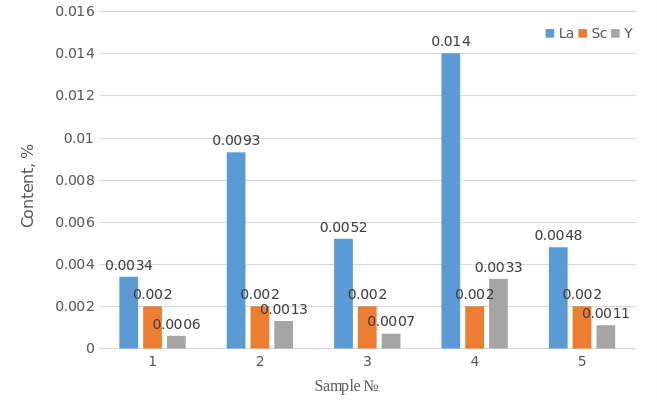
\includegraphics[width=0.7\textwidth]{assets/1084}
	\caption*{Figure 6 - Rare Earth Metal Content in Coal Ash Slag Waste from the Shubarkol Deposit}
\end{figure}

\begin{multicols}{2}
The investigation of this fly ash has focused on identifying the content
of rare earth metals such as lanthanum, scandium, and yttrium. The
obtained results confirm that the extraction of rare metals from
secondary sources, including waste processing, represents a promising
approach. This helps to reduce the risk of increasing waste volumes and
creates a basis for the development of an independent raw material base.

The coal reserves of the Karaganda Coal Basin have not been adequately
studied for the content of rare earth metals, and their resources can
only be partially assessed. However, in the case of the Shubarkol
deposit in Central Kazakhstan, where reserves exceed 1 billion tons,
significant amounts of rare earth metals have been found during coal
combustion at thermal power plants. The content of yttrium is up to 100
g/t, scandium - 64 g/t, dysprosium - 384 g/t, and gadolinium - 335 g/t.
These data indicate a significant potential for the extraction of rare
earth metals from coal ash slag at thermal power plants.

Сonclusions. The article discusses the significance of coal mining and
comprehensive processing in the context of Kazakhstan\textquotesingle s
Development Concept of the Fuel and Energy Industry and the transition
to a "Green Economy." It emphasizes the importance of researching and
developing environmentally friendly technologies for coal extraction,
combustion, and processing.

Rare Metal Potential: The study emphasizes the largely untapped
potential of rare metals in coal and its by-products. While germanium
and gold are currently extracted on an industrial scale, technologies
for extracting gallium, scandium, rare earth metals, and other metals
have been developed.

Environmental Concerns: The article underscores the environmental
threats posed by ash dumps from local thermal power plants. These dumps
can lead to air and soil pollution, posing risks to human health and
ecosystems.

Economic and Environmental Benefits of Waste Utilization: Utilizing
waste from coal combustion not only addresses environmental concerns but
also offers economic benefits. Secondary waste processing can reduce
expenses on storage and lead to the extraction of rare and rare earth
metals, contributing to economic efficiency.

Rare Earth Metals in Coal Deposits: The Shubarkol deposit in Central
Kazakhstan is highlighted for its significant reserves of rare earths,
including scandium, dysprosium, and gadolinium. These metals can be
extracted during coal combustion at thermal power plants.

Research and Development: The article stresses the importance of further
research and development in the extraction of rare metals from coal and
its by-products. It suggests that existing extraction methods have low
efficiency, limiting investment attractiveness.

Overall, the study underscores the potential of coal deposits not only
as sources of fuel but also as valuable reservoirs of rare elements. It
advocates for the development of technologies to extract these elements
efficiently, thereby mitigating environmental impacts and maximizing
economic benefits.
\end{multicols}

\begin{center}
{\bfseries References}
\end{center}

\begin{noparindent}{2}
1.Ob utverzhdenii Kontseptsii razvitiya toplivno-energeticheskogo
kompleksa Respubliki Kazakhstan na 2023 -- 2029 gody. postanovleniya
Pravitel\textquotesingle stva RK ot 28.03.2023 № 260. {[}in Russ.{]}

2.Khoroshavin, L. B. Osnovnye tekhnologii pererabotki promyshlennykh i
tverdykh kommunal\textquotesingle nykh otkhodov : {[}ucheb. posobie{]} /
L. B. Khoroshavin, V. A. Belyakov, E. A. Svalov ; {[}nauch. red. A. S.
Noskov{]} ; M-vo obrazovaniya i nauki Ros. Federatsii, Ural. feder.
un-t. -- Ekaterinburg : Izd-vo Ural. un-ta, 2016. -- 220 s. ISBN
978-5-7996-1747-9. {[}in Russ.{]}

3.Kryukov V.A., Yatsenko V.A., Kryukov Ya.V.
Redkozemel\textquotesingle naya promyshlennost\textquotesingle{} -
realizovat\textquotesingle{} imeyushchiesya vozmozhnosti//Gornaya
promyshlennost\textquotesingle. 2020.- № 5.-S.68-84. {[}in Russ.{]}

DOI:~http://dx.doi.org/10.30686/1609-9192-2020-5-68-84

4.Arbuzov S.I., Chekryzhov I.Yu., Tarasenko I.A.
Redkometall\textquotesingle nyi potentsial uglei Sibiri i
Dal\textquotesingle nego Vostoka Rossii i perspektivy ego osvoeniya//
Vestnik DVO RAN.- 2023.- No 5. S.31-51. {[}in Russ.{]} DOI:
10.37102/0869-7698\_2023\_231\_05\_3

5.Adeeva L. N., Borbat V. F. Zola TETs perspektivnoe
syr\textquotesingle e dlya promyshlennosti// Vestnik Omskogo
universiteta.- 2009.- № 2.- S. 141-151{[}in Russ.{]}

6.Mausymbaeva A.D. Izuchenie osobennostei veshchestvennogo sostava i
napravleniya kompleksnogo ispol\textquotesingle zovaniya uglei
mestorozhdeniya Shubarkol\textquotesingle{}
(Tsentral\textquotesingle nyi Kazakhstan). dissertaciya na soiskanie
stepeni doktora filosofii. Karaganda. 2020. 152 s.
https://www.geokniga.org/bookfiles/geokniga-izuchenie-osobennostey-veshchestvennogo-sostava.pdf

7. Maslov М., Komarova S., Kunilova I., Gol\textquotesingle berg G.
Obzor metodov kontrolya soderzhaniya redkozemel\textquotesingle nykh
elementov i granulometricheskogo sostava zoly szhiganiya uglei.// /
Rol\textquotesingle{} tehnicheskogo regulirovanija i standartizacii v
jepohu cifrovoj jekonomiki : sbornik statej uchastnikov IV
Mezhdunarodnoj nauchno-prakticheskoj konferencii molodyh
uchenyh.-Ekaterinburg.-2022.- S.214-224.{[}in Russ.{]}

8. Bazarova E. A. Opredelenie redkikh i redkozemel\textquotesingle nykh
elementov v baddeleitovom kontsentrate metodom mass-spektrometrii s
induktivno svyazannoi plazmoi / E.A. Bazarova, A.I. Novikov, S.V.
Drogobuzhskaya // Trudy KNTs RAN. Khimiya i materialovedenie. Vyp. 1. --
2017, № 5 (8). -- S.27-34. {[}in Russ.{]}

9.Nikolaeva I. V. Opredelenie osnovnykh i primesnykh elementov v
silikatnykh porodakh metodom

mass-spektrometrii s induktivno-svyazannoi
plazmoi posle splavleniya s LiBO2 / I.V. Nikolaeva, S.V. Palesskii, O.S.
Chirko, S.M. Chernonozhkin // Analitika i kontrol\textquotesingle. --
2012. -- T. 16, № 2. -- S. 134-142. {[}in Russ.{]}

10.Zhernokleeva K. V. Analiz redkozemel\textquotesingle nykh metallov i
ikh oksidov atomno-emissionnym i mass-spektral\textquotesingle nym
metodami s induktivno-svyazannoi plazmoi: Avtoref. Dis\ldots kandidata
tekhnicheskikh nauk / K.V. Zhernokleeva. -- M.- 2011.-34 s. {[}in
Russ.{]}

11.Panteeva S. V. Osobennosti opredeleniya soderzhanii ryada elementov v
gornykh porodakh razlichnogo sostava metodami mass-spektrometrii s
induktivno svyazannoi plazmoi i rentgenofluorestsentnogo analiza / S.V.
Panteeva // Analitika i kontrol\textquotesingle{} -- 2009. -- T. 13, №
4. -- S. 184-192. {[}in Russ.{]}

12.GOST R 54237-2010. Toplivo tverdoe mineral\textquotesingle noe.
Opredelenie khimicheskogo sostava zoly metodom atomno-emissionnoi
spektrometrii s induktivno svyazannoi plazmoi. Data vvedeniya:
2010-12-23. -- M.: Standartinform, 2012. -- 16 s. {[}in Russ.{]}

13. GOST R 57923-2017 (ISO 24235:2007). Kompozity keramicheskie.
Opredelenie granulometricheskogo sostava keramicheskih poroshkov metodom
lazernoj difrakcii: data vvedeniya 2017-11-08. -- Izd
oficial\textquotesingle noe. -- M.: Standartinform, 2017. -- 11 s.

14.Silachev I. Yu. Kompleksirovanie instrumental\textquotesingle nogo
neitronno-aktivatsionnogo i rentgenofluorestsentnogo analiza dlya
opredeleniya soderzhaniya redkozemel\textquotesingle nykh elementov v
geologicheskikh obraztsakh / I.Yu. Silachev // Zhurnal analiticheskoi
khimii.-2020.- T. 75, № 7. -- S. 616-628. DOI:
10.31857/S0044450220070142

15.Miller, R.J. Schaetzl. Precision of Soil Particle Size Analysis using
Laser Diffractometry / B.A // Soil Science Society of America Journal. -
2012.-V. 76 (5).- P. 1719-1727. DOI:10.2136/sssaj2011.0303 {[}in Eng.{]}

16.Ermagambet B.T., Nurgaliev N.U., Kasenova Zh.M., Urlibai R.K., Bolat
O.S., Semenova Ya.A. Tekhnologiya pererabotki zoloshlakovykh otkhodov
Kazakhstana// 2020 S. 82-86

URI:~http://nur.nu.edu.kz/handle/123456789/4942.{[}in Russ.{]}

17.Zalelova A. M., Ibraev M. K. Podbor podkhodyashchikh dlin voln dlya
opredeleniya massovoi doli

redkozemel\textquotesingle nykh elementov v
probakh uglei i produktakh ikh pererabotki polukolichestvennym
spektral\textquotesingle nym atomnoemissionnym metodom// Electronic
journal, S.1-14 http://elib.kstu.kz/

http://elib.kstu.kz/fulltext/temat/PODBOR\%20PODHODYASHCHIH\%20DLIN\%20VOLN.pdf

18 Ibraev M.K., Dauletzhanova ZH.T., Zalelova A.M., Rahimzhanova Z.A.
Issledovanie uglei na nalichie

redkozemel\textquotesingle nykh
metallov// Colloquium-journal. - 2017. - № 11-2. - S. 18-21;

https://colloquium-journal.org/wp-content/uploads/2017/11/Colloquium-journal-2017-11-2.pdf
\end{noparindent}

\emph{{\bfseries Information about the authors}}

\begin{noparindent}
Dauletzhanova Zh. T. - PhD, associate Professor of the Chemistry,
Chemical Technology and ecology department, Kazakh University of
Technology and Business named after K. Kulazhanov, Astana, Kazakhstan,

kaliyeva\_zhanna@mail.ru;

Nurtay Zh. T.- PhD, Head of the Department of Chemistry and Chemical
Technology and ecology department, Kazakh University of Technology and
Business named after K. Kulazhanov, Astana, Kazakhstan,

zhadira\_nurtai@mail.ru
\end{noparindent}

\emph{{\bfseries Сведения об авторах}}

\begin{noparindent}
Даулетжанова Ж. Т. -- PhD, асоциированный профессор кафедры Химии,
химической технологии и экологии Казахского университета технологии и
бизнеса им. К. Кулажанова, Астана, Казахстан,

kaliyeva\_zhanna@mail.ru;

Нуртай Ж. Т.- PhD, заведующий кафедрой Химии, химической технологии и
экологии Казахского университета технологий и бизнеса им. К. Кулажанова,
к.э.н., Астана, Казахстан, zhadira\_nurtai@mail.ru
\end{noparindent}
